\documentclass{../HM}
\newcommand\course{HM 2}
\newcommand\hwnumber{10}
\usepackage{gauss}
\usepackage{tikz}
\usepackage{pgfplots}

\newcommand{\mue}{m_{\textit{ü}}}
\begin{document}
	\begin{enumerate}
		\item[10.2] Eine (idealisiert homogene) Kette der Länge $l$ liegt auf einem horizontalen, reibungsfreien Tisch, wobei ein Stück Kette der Länge $a$ über den Rand hängt. Wie lange dauert es, bis die kette vom Tisch geglitten ist?\\\\
		Hinweis: Bezeichne die Gesamtmasse der Kette mit $m$ und die Länge des überhängenden Stücks zur Zeit $t$ mit $y(t)$. Berechne die Masse $\mue(t)$ des überhängenden Stücks zur Zeit $t$. Die Gravitationskraft $\mue(t)g$ muss dann gleich $F=m\ddot{y}(t)$ sein.
		
		\begin{eqnn}
			\eqnf{\mue(t)}{y(t)\frac{m}{l}}
			\eqnf{F}{m\ddot{y}(t)}
			\eqn{F}{\mue(t)g}
			\geqn[][\Rightarrow]{m\ddot{y}(t)}{\feq}{\mue(t)g}
			\eqn{\ddot{y}(t)-y(t)\frac{g}{l}}{0}
			\eqntext{Homogene Differentialgleichung lösen:}
			\eqn[][\Rightarrow]{p(\lambda)}{\lambda^2-\frac{g}{l}=0}
			\eqn[][\Rightarrow]{\lambda}{\pm\sqrt{\frac{g}{l}}}
			\eqn[][\Rightarrow]{y(t)}{c_1e^{t\sqrt{\frac{g}{l}}}+c_2e^{-t\sqrt{\frac{g}{l}}}}
			\eqntext{Bedingung $y(0)=a$ einsetzen, da die Länge des überhängenden Stücks der Kette zum Zeitpunkt $t=0\to a$ ist:}
			\eqn[][\Rightarrow]{c_1+c_2}{a}
			\eqn{c_1}{a-c_2}
			\eqn[][\Rightarrow]{y(t)}{(a-c_2)e^{t\sqrt{\frac{g}{l}}}+c_2e^{-t\sqrt{\frac{g}{l}}}}
			\eqnspace
			\eqntext{Da die Kette eine idealisiert homogene Verteilung ihres Gewichts aufweist, folgt $\dddot{\mue}(t)\feq 0$:}
			\eqnf{\mue(t)}{y(t)\frac{m}{l}}
			\eqn[][\Rightarrow]{\dot{\mue}(t)}{\sqrt{\frac{g}{l}}\frac{(a-c_2)m}{l}e^{t\sqrt{\frac{g}{l}}}-\sqrt{\frac{g}{l}}\frac{c_2m}{l}e^{-t\sqrt{\frac{g}{l}}}}
			\eqn[][\Rightarrow]{\ddot{\mue}(t)}{\frac{mg}{l^2}\left((a-c_2)e^{t\sqrt{\frac{g}{l}}}+c_2e^{-t\sqrt{\frac{g}{l}}}\right)}
			\eqn[][\Rightarrow]{\dddot{\mue}(t)}{\frac{mg}{l^2}\sqrt{\frac{g}{l}}\left((a-c_2)e^{t\sqrt{\frac{g}{l}}}-c_2e^{-t\sqrt{\frac{g}{l}}}\right)\feq 0}
			\eqn{0}{ae^{t\sqrt{\frac{g}{l}}}-c_2e^{t\sqrt{\frac{g}{l}}}-c_2e^{-t\sqrt{\frac{g}{l}}}}
			\eqn{0}{-c_2(e^{-t\sqrt{\frac{g}{l}}}-e^{t\sqrt{\frac{g}{l}}})}
			\eqn{c_2}{0}
			\eqntext{$c_2$ in $y$ einsetzen:}
			\eqn[][\Rightarrow]{y(t)}{ae^{t\sqrt{\frac{g}{l}}}}
			\eqntext{Zum Zeitpunkt des Abrutschen, muss $y(t)=l$ betragen (Die gesamte Kette ist vom Tisch gerutscht):}
			\geqnf{ae^{t\sqrt{\frac{g}{l}}}}{\feq}{l}
			\eqn{t\sqrt{\frac{g}{l}}}{\ln(\frac{l}{a})}
			\eqn{t}{\frac{\ln(\frac{l}{a})}{\sqrt{\frac{g}{l}}}}
		\end{eqnn}
		
		\item[10.3] Löse die folgenden Anfangswertaufgaben:
		\begin{enumerate}
			\item $\ddot{y}+2\dot{y}-3y=e^{2t}, y(0)=0, \dot{y}(0)=1$.
			\begin{eqnn}
							\eqnf{P(\lambda)}{\lambda^2+2\lambda-3=0}
				\eqn{\lambda}{-1\pm2}
				\eqn[][\Rightarrow]{\lambda_1}{-3,}
				\eqnf{\lambda_2}{1}
				\eqnspace
				\eqntext{eine homogene Lösungsbasis finden:}
				\eqn[][\Rightarrow]{y_H(t)}{c_1e^t+c_2e^{-3t}}
				\eqnf{\ddot{y}+2\dot{y}-3y}{0}
				\eqnspace
				\eqntext{eine spezielle Lösungsbasis finden:}
				\eqntext{da $b(t)=2^{2t}$ mit $\lambda=2\neq\lambda_1,\lambda_2$ liegt kein Resonanzfall vor:}
				\eqn{y_s(t)}{c_3e^{2t}}
				\eqn{\dot{y}_s(t)}{2c_3e^{2t}}
				\eqn{\ddot{y}_s(t)}{4c_3e^{2t}}
				\eqntext{in Ausgangsgleichung einsetzen:}
				\eqn[][\Rightarrow]{5c_3e^{2t}}{e^{2t}}
				\eqn{c_3}{\frac{1}{5}}
				\eqntext{$c_3$ in $y_s$ einsetzen:}
				\eqn[][\Rightarrow]{y_s(t)}{\frac{1}{5}e^{2t}}
				\eqn[][\Rightarrow]{y(t)}{c_1e^t+c_2e^{-3t}+\frac{1}{5}e^{2t}}
				\eqn{\dot{y}(t)}{c_1e^t-3c_2e^{-3t}+\frac{2}{5}e^{2t}}
			\end{eqnn}
			\begin{eqnn}
				\eqntext{Anfangswertbedingungen einsetzen:}
				\eqn[$y(0)=0$][]{c_1+c_2}{\frac{1}{5}}
				\eqn[$\dot{y}(0)=1$][]{c_1-3c_2}{\frac{3}{5}}
				\eqn[][\Rightarrow]{\m{1&1\\1&-3}[\add[\cdot(-1)][+]{0}{1}]c}{\m{-\frac{1}{5}\\\frac{3}{5}}}
				\eqn{\m{1&1\\0&-4}c}{\m{-\frac{1}{5}\\\frac{4}{5}}}
				\eqn[][\Rightarrow]{c_2}{-\frac{1}{5}}
				\eqn[][\Rightarrow]{c_1}{0}
				\eqntext{$c_1,c_2$ in $y$ einsetzen:}
				\eqn[][\Rightarrow]{y(t)}{\frac{1}{5}\left(e^{3t}-e^{-3t}\right)}
			\end{eqnn}
			
			\item $\ddot{y}+y=t+2\cos(t), y(\pi)=2\pi, \dot{y}(\pi)=\pi$.
			\begin{eqnn}
				\eqnf{P(\lambda)}{\lambda^2+1=0}
				\eqn{\lambda}{\pm i}
				\eqnspace
				\eqntext{eine homogene Lösungsbasis finden:}
				\eqnf{y_H(t)}{c_1e^{it}+c_2e^{-it}}
				%\eqn{y_H(t)}{c_1\sin(t)+c_2\sin(-t)}
				%\eqn{y_H(t)}{c_1\cos(t)+c_2\cos(-t)}
				\eqnspace
				\eqntext{spezielle Lösungsbasen finden:}
				\eqn[$y_{s1}$][\Leftarrow]{\ddot{y}+y}{t}
				\eqntext{da $\lambda=0\neq\lambda_1,\lambda_2$ liegt kein Resonanzfall vor:}
				\eqn[][\Rightarrow]{y_{s1}}{c_3+c_4t}
				\eqn{\dot{y}_{s1}}{c_4}
				\eqn{\ddot{y}_{s1}}{0}
				\eqntext{in Ausgangsgleichung ($y_{s1}$) einsetzen:}
				\eqn{c_3+c_4}{t}
				\eqn[][\Rightarrow]{c_3}{0,}
				\eqnf{c_4}{1}
				\eqntext{$c_3,c_4$ in $y_{s1}$ einsetzen:}
				\eqn[][\Rightarrow]{y_{s1}}{t}
				\eqnspace
				\eqn[$y_{s2}$][\Leftrightarrow]{\ddot{y}+y}{2\cos(t)=\Re(2e^{it})}
				\eqntext{durch $\lambda=i=\lambda_1$ liegt ein Resonanzfall einer einfachen Nullstelle vor. Dadurch muss ein Vorfaktor $t$ hinzugefügt werden:}
				\eqn[][\Rightarrow]{\widetilde{y}_{s2}(t)}{cte^{it}}
				\eqn{\widetilde{\dot{y}}_{s2}(t)}{ce^{it}(ti+1)}
				\eqn{\widetilde{\ddot{y}}_{s2}(t)}{ce^{it}(2i-t)}
				\eqntext{in Ausgangsgleichung einsetzen:}
				\eqn{2ci}{2}
				\eqn{c}{-i}
				\eqn[][\Rightarrow]{\widetilde{y}_{s2}}{-ite^{it}}
				\eqn{y_{s2}}{\Re(\widetilde{y}_{s2})}
				\eqn{y_{s2}}{t\sin(t)}
				\eqntext{Da $y=y_H+y_s$:}
				\eqn[][\Rightarrow]{y(t)}{c_1e^{it}+c_2e^{-it}+t+t\sin(t)}
				\eqn{\dot{y}(t)}{c_1ie^{it}-c_2e^{-it}+1+\sin(t)+t\cos(t)}
				\eqntext{Anfangswertbedingungen einsetzen:}
				\eqn[$y(\pi)=2\pi$][]{-ic_1-c_2+\pi}{2\pi}
				\eqn{ic_1+c_2}{-\pi}
				\eqn[$\dot{y}(\pi)=\pi$][]{-ic_1+c_2+1-\pi}{\pi}
				\eqn{-ic_1+c_2}{2\pi-1}
				\eqn[][\Rightarrow]{\m{-i&-1\\-i&1}[\add[\cdot(-1)][+]{0}{1}]c}{\m{-\pi\\2\pi-1}}
				\eqn{\m{-i&-1\\0&2}}{\m{-pi\\3\pi-1}}
				\eqn[][\Rightarrow]{c_2}{\frac{1}{2}(\pi-1),}
				\eqnf{c_1}{\frac{i}{2}(-\pi-1)}
				\eqntext{$c_1,c_2$ in $y$ einsetzen:}
				\eqn{y(t)}{\frac{1}{2}(-i(\pi+1)e^{it}+(\pi-1)e^{-it})+t(\sin(t)+1)}
			\end{eqnn}
		\end{enumerate}
		
		\item[10.4]
		\begin{enumerate}
			\item Stelle eine homogene lineare Differentialgleichung 3.Ordnung auf, so dass eine Lösungsbasis gegeben ist durch $y_1(t)=1, y_2(t)=t, y_3(t)=e^t$.
			
			\begin{eqnn}
				\eqntext{$\lambda_1=1$, $\lambda_2=0$ doppelte Nullstelle}
				\eqn[][\Rightarrow]{p(\lambda)}{(\lambda-1)\lambda^2}
				\eqn[][\Rightarrow]{y'''-y''}{0}
			\end{eqnn}
			
			\item Finde eine homogene lineare Differentialgleichung, so dass $y_1:\R\to\R, y_1(t)=t$ und $y_2:\R\to\R, y_2(t)=\sin(t)$ Lösungen sind.
			
			
			\begin{eqnn}
				\eqntext{$y_1=t=te^{0t}$, $y_2=\sin(t)=\Im(e^{it})$}
				\eqn[][\Rightarrow]{\lambda_1}{0 \text{ doppelte Nullstelle}}
				\eqn[][\Rightarrow]{\lambda_2}{\pm i}
				
				\eqn[][\Rightarrow]{p(\lambda)}{\lambda^2(\lambda^2+1)}
				\eqn[][\Rightarrow]{y''''+y''}{0}
			\end{eqnn}
			
			\item Warum ist es in (b) unmöglich, eine homogene lineare Differentialgleichung 2.Ordnung aufzustellen, selbst wenn man zeitabhängige Koeffizienten zulässt, d.h. wenn man eine Differentialgleichung der Form
			$$\ddot{y}+a_1(t)\dot{y}+a_0(t)y=0$$\\
			sucht, mit $a_0,a_1:\R\to\R$?\\
			
			$$\md{t&\sin(t)\\1&\cos(t))}= t\cos(t)-\sin(t)$$
			
			Im Fall $t=0$ ist die Wronski-Determinante gleich 0\\
			Daraus folgt, dass die gegebenen Lösungen nicht linear unabhängig sind. Und da eine lineare Differentialgleichung 2. Ordnung dieser Art, zwei linear unabhänige Lösungen hat wissen wir, dass es keine lineare Differentialgleichung 2. Ordnung mit den gegebenen Lösungen gibt.
			
			\item Warum ist es in (b) auch nicht möglich, eine homogene lineare Differentialgleichung 3.Ordnung aufzustellen, selbst wenn man zeitabhängige Koeffizienten zulässt?
			
			
			$$\md{t&\sin(t)&a\\1&\cos(t)&b\\0&-\sin(t)&c}=t\cos(t)c-\sin(t)a+\sin(b)t-c\sin(t)$$
			Im Fall $t=0$ ist die Wronski-Determinante gleich 0\\
			Wie in (d) folgt hieraus, dass es keine lineare Differentialgleichung 3.Ordnung mit den gegebenen Lösungen gibt.\\
			
			\item[] Hinweis zu (c) und (d): Wronski-Determinante, Satz 10.1, $n$ Lösungen $y_1,\hdots,y_n$ einer homogenen linearen Differentialgleichung $n$.Ordnung sind genau dann linear unabhängig, wenn
			$$\md{
				y_1(t)&y_2(t)&\hdots&y_n(t)\\
				\dot{y}_1(t)&\dot{y}_2(t)&\hdots&\dot{y}_n(t)\\
				\vdots&\vdots&\ddots&\vdots\\
				y^{(n-1)}_1(t)&y^{(n-1)}_2(t)&\hdots&y^{(n-1)}_n(t)
			}\neq 0$$\\
			für alle $t$. Was passiert hier für $t=0$?
		\end{enumerate}
		
		\item[10.5] Eine gedämpfte Schwingung ohne Anregung sei modelliert durch
		$$\ddot{y}+a\dot{y}+4y=0, \quad y(0)=5,\quad \dot{y}(0)=-1$$\\
		Bestimme den Parameter $a>0$ so, dass gerade der aperiodische Grenzfall eintritt, und berechne die Lösung für diesen Fall. Stelle den zeitlichen Verlauf der Schwingungen graphisch dar.
		\begin{eqnn}
			\eqntext{Aus dem Ansatz für Kritisch gedämpfte Fälle:}
			\eqn[][\Rightarrow]{\ddot{y}+2p\dot{y}+\omega^2y}{\ddot{y}+a\dot{y}+4y}
			\eqn[][\Rightarrow]{a}{2p}
			\eqn[][\Rightarrow]{\omega}{2}
			\eqn[][\Rightarrow]{y}{c_1e^{-2t}+c_2te^{-2t}}
			\eqntext{Anfangswerte einsetzen:}
			\eqn[][\Rightarrow]{c_1}{5}
			\eqn[][\Rightarrow]{-1}{-2c_1+c_2}
			\eqn{c_2}{9}
			\eqn[][\Rightarrow]{y}{e^{-2t}(t+9t)}
		\end{eqnn}
		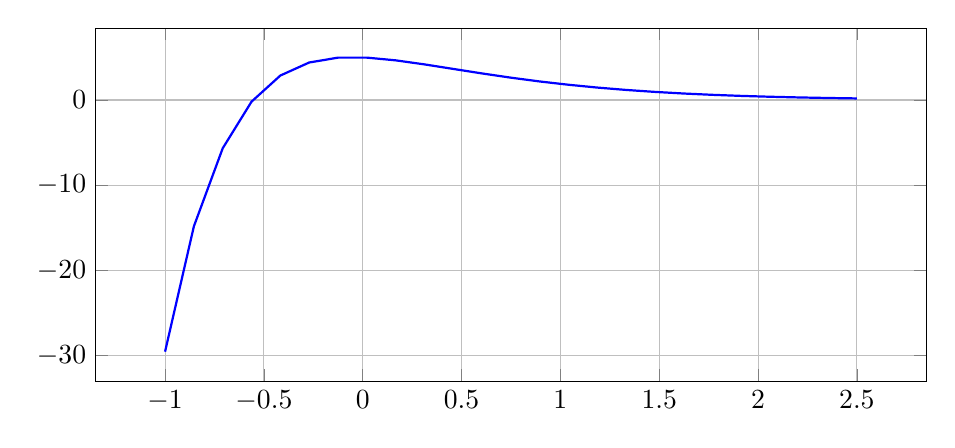
\begin{tikzpicture}
			\begin{axis}[
				grid = both,
				width = \textwidth,
				height = 0.5\textwidth
				]
				\addplot[domain = -1:2.5,blue,thick] {exp(-2*x)*(5+9*x)};
			\end{axis}
		\end{tikzpicture}
	\end{enumerate}
\end{document}
